
%As said before, typically, stating the MAPF problem begins with introducing the graph and constraints related to how agents are allowed to move on that graph. On the contrary, we wish to describe how agents and their moves are modeled in non-constrained environment (i.e. in 2D or 3D) and only then introduce a graph discretization of the problem.

%Consider a group of $n$ homogeneous agents operating in the shared environment which is a closed subset of the Euclidean 2-dimensional or 3-dimensional space, e.g. a bounded rectangle $W \in \mathbb{R}^2$. Without the loss of generality we will assume 2D workspace further in the paper. The environment is composed of the free space and the obstacles: $W = W_{free} + W_{obs}$. All agents have the same shape and size and each agent is characterized by its position $\textbf{p}=(x, y)$. An agent can move from one location to the other following an arbitrary shaped curve (line segment in the simplest case) connecting the move's endpoints.

%We assume that the two collision detection functions are given:
%\begin{itemize}
%    \item the one that detects collision w.r.t. static obstacles:
    
%    $col_{st}: W \rightarrow \{true, false\}$;
%    \item the one that detects inter-agent collisions:
    
%    $col_{ia}: W \times W \rightarrow {true, false}$.
%\end{itemize}

%In the simplest case, e.g. when the circular agents are considered, $col_{st}$ returns true if the distance between the position of an agent and the closest point in $W_{free}$ is less than the agent's radius; and $col_{ia}$ returns true if the distance between the positions of two agents is less than the sum of their radii.

%The path for an agent $i$ is defined as the mapping of the timeline to the workspace: $\pi: T \rightarrow W$, where $T=[0, + \infty)$.

%This definition of the path is the ``most unconstrained one'' as no limitations are imposed on how the agent might move, i.e. all sorts of acceleration/decelleartion are allowed, instantaneous direction changes are allowed, no constraints are imposed on the curvature of the path etc. Practice-wise this assumption never holds as only certain types of moves can be performed by the agents due to kinematic/dynamic constraints. Thus it is natural to introduce a notion of action and to constrain a path to be composed only of the actions in a certain order. Formally, action is, like a path, a mapping from time moments to workspace: $a: [t_b, t_e) \rightarrow W$, where $t_b, t_e \in T$ and $t_e<t_b$. And the path can now be defined as a sequence of actions: $\pi = \langle a_1, a_2, ..., a_k\rangle$, s.t. $t_e(a_j)=t_b(a_{j+1}$ and $a_j(t_e)=a_{j+1}(t_b)$. The conditions insure that the consecutive actions are well-aligned in time-space, i.e. the next action starts immediately after the previous one and in the same location of the workspace.


%We are considering cooperative pathfinding for non-point translating non-rotating agents in 2D workspaces. we consider all agents (1) to be of the same shape and size, i.e. open disks, (2) to move with the same (constant) speed, and (3) to be constrained to the same roadmap of the environment, i.e. there is a single graph $G=(V, E)$ whose vertices correspond to the locations agents can occupy (and wait in them) and edges correspond to straight-line trajectories the agents traverse when moving from one location to the other. Inertial effects are neglected and agents start/stop moving instantaneously. Duration of a move is translation speed times the length of the edge. Duration of the wait action can be any positive real number. 
%Prior work referred to this setting as \mapfr~\cite{walker2018extended}.
%Having that said, the problem we are considering is analogous to the one introduced by Walker et al.~\shortcite{walker2018extended} and dubbed \mapfr.

%Note that the \ccbs algorithm we propose in this work is not limited to assumptions (1), (2), and (3) described above, e.g., it can handle agents moving with different speeds, using different roadmaps, and having complex shapes and sizes. We make these assumptions only to simplify exposition. % provided with the appropriate collision detection procedure. It’s also extensible for 3D environments.Assumptions \textit{i}, \textit{ii}, and \textit{iii}For the sake of simplicity \konstantin{i think we need to say the following somewhere: may be here in text, may be in the footnote, maybe in the next section}Please note that the algorithm we are about to propose is not limited to \textit{i}), \textit{ii}) and \textit{iii}) assumptions, e.g. it can handle open-disk agents moving with different speeds and each of them using its own roadmap of the environment. Moreover it can be used for agents with different (complex) shapes and sizes provided with the appropriate collision detection procedure. It’s also extensible for 3D environments.

%The set of vertices $V$ represents a set of locations that the agents can occupy. We assume that any two agents, when standing still, can occupy any two vertices in the graph without colliding, i.e. their bodies will not overlap. For graphs based on grids and disk-shaped agents, this means the radius of every agent is less than or equal to half of the cell size.
%\begin{figure}
%\centering
%    \centering
%    \includegraphics[width=0.75\columnwidth]{RegularGraph.png}
%    \caption{}
%    \label{fig:reggrapph}
%\end{figure}
% Agents' actions
%When an agent is at a location $v\in V$, it can either  perform a \emph{move} action or a \emph{wait} action. 
%A move action moves the agent along an edge $(v,v')\in E$, and a wait action means the agents stays in $v$. 
%Every action has a \emph{duration}. The duration of a move action is the weight of the edge the agent is traversing. The duration of a wait action can be any positive real value. Thus, every agent has an infinite number of wait moves in every location. 
 
%\roni{I am missing more about the geometric prospective of the domain.  	That is, instead of a graph, the domain is actually represented by some terrain,  	and the graph is just set on that terrain. Probably there's such a definition in prior work on any-angle stuff.}





% END OF COPY AND PASTE FROM WORKSHOP PAPER


\subsection{Action execution in continuous time and space}
\textbf{K: This section might be of some value (but not sure)}

The distinctive feature of the considered problem statement is that the agents execute the actions of their plans in continuous time and space. By saying so we mean that for every agent $i$ and its plan $\pi_i$, and for every moment $t \in T=[0, +\infty)$ there exist a distinct $(x, y)$ location on the edge (or vertex) of the graph that is occupied by $i$ at $t$. In other words we are not blocking the edge entirely for the time the agent is traversing it.

Consider an example depicted on Figure \ref{fig:example} and assume the plan for the blue agent is $G \rightarrow H \rightarrow C \rightarrow D$ without any waits. Then, assuming that the moving speed equals 1, the agent will start traversing the edge $H \rightarrow C$ at time 2 and at time moment, say, $3.3$ it will be at the $(XXXX, YYY)$. This means that other agents, e.g. the red one, can be at this time moment anywhere on the edge $F \rightarrow I$ (the edge is not blocked), as the distance between the center of the blue agent and any point on the edge $F \rightarrow I$ is greater that $2r=2*0.5=1$.

\textbf{K: Maye some picture here showing (by the arrow) the position of the blue agent at time 3.3}

\section{Conflict-Based Search with Continuous Time and Space}




\subsection{Related \mapf Problems}

\roni{Below I describe almost word-to-word the models used by Thayne and Liron. Let's discuss this next time we talk}
% MAPFR
Walker et al.~\cite{walker2018extended} are, to the best of our knowledge, the first to extend the definition of \mapf to consider non-unit edge costs. 
They introduced the \mapfr problem, which is different from classical \mapf in the following ways. 
In \mapfr, every edge $e=(v,v')$ in the underlying graph $G$ is associated with a positive weight $w(e)\in \mathbb{R}_{>0}$ that represents the duration it takes an agent to move from $v$ to $v'$. 
Every location $v\in V$ is associated with a unique coordinate in a metric space, denoted $\coord(v)$. 
An agent is a circle with a non-zero volume. 
When the location of an agent is $v$, it means the center of the agent is located at $\coord(v)$. 
When an agent moves along an edge $(v,v')$, it means
its center moves along a straight line from $\coord(v)$ to $\coord(v')$ in a constant velocity motion. 
There is a conflict between two single-agent plans iff the volumes of ``one or more agents overlap at the same instant in time''~\cite{walker2018extended}. This can be detection by using standard collision detection techniques~\cite{helpHere}. 

% Limitation of MAPFR
Walker et al.~\cite{walker2018extended} proposed the Extended Increasing Cost Tree Search (E-ICTS) algorithm for finding bounded-suboptimal solutions to \mapfr problems. 
However, the definition of \mapfr does not specify the duration of wait actions. In their implementation, wait actions had a fixed small duration, which E-ICTS accepts as a parameter. 


% Multi-agent motion planning
Cohen et al.~\cite{cohen} proposed a relevant extension of classical \mapf that they called \emph{multi-agent motion planning} (MAMP). In MAMP, each agent is associated with a graph $G_i=(V_i,E_i)$. 
A vertex in $V_i$ represents a possible \emph{state} of agent $i$, where a state of an agent represents its location as well as other relevant features such as orientation and steering angle. 
An edge $e_i=(v,v')\in E_i$ represents a kinodymaically feasible motion of agent $i$ from state $v$ to state $v'$, 
and the weight of an edge is the duration of performing this motion.
%Importantly, the sets of cells associates with states of different agents may intersect, thereby indicating a potential conflict. 
The agents in MAMP move in an \emph{environment} represented by a list of cells $\mathcal{C}$. 
Every state $v\in V_i$ of an agent $i$ is associated with a set of cells in $\mathcal{C}$, representing the cells occupied by that agent when in state $v$. 
Every edge $e_i=(v,v')\in E_i$ is associated with a multiset of cells in $\mathcal{C}$. 
Each cell in this multiset is associated with a time interval indicating the time interval in which this cell is occupied when agent $i$ moves from $v$ to $v'$.

% Limitation of MAMP
Cohen et al.~\cite{cohen2019optimal} proposed an optimal and a bounded-suboptimal algorithm for solving MAMP problems, based on Conflict-Based Search (CBS)~\cite{sharon2015conflict}. Their algorithm, called CBS-CT, is designed to consider continuous time. However, it relies on the discretizes representation of the environment into a set of cells ($\mathcal{C}$). 


\roni{I'm going ahead and editting the below following the terminology above and my understanding of our problem as a \mapfr problem. 
The original text is in backup-main.alt file, so don't worry, we can revert easily.}
\roni{There was wonderful text there about 3 assumptions and how we lift them. I think much of that should go in the introduction.}


\section{Problem Definition}

It can be said that CBS-CT~\cite{cohen2019optimal} deals with continuous time but with a discrete motion model, 
while E-ICTS~\cite{walker2018extended} deals with continuous motion but discretize wait times. We focus on the more general setting in which motion between vertices is continuous and wait time can also be any real number. 



%5TODO: Konstantin
Typically the \ac{MAPF} problem is formulated as a graph search problem, i.e. all agents are confined to the graph $G=(V, E)$, which vertices correspond to the locations in the environment and the edges -- to the feasible transitions between the locations. The time is discretized into the timesteps and it is assumed that at each time step an agent can either wait at the vertex or move from this vertex to some of its neighbors, following a certain edge. The path for an agent is formally a mapping from the timesteps to the graph vertices: $\pi = T \rightarrow V$, where $T=[0, 1, 2, ...]$, s.t. each two consecutive timesteps are mapped either to the same vertex (the agent is waiting) or to the two adjacent vertices (the agent is moving). Because the time is discretized an agent can be though of as teleporting from one vertex to the other (or to the same vertex, in case of the wait action).

In case only one agent is present in the environment (on the graph), each its path is feasible, i.e. no collision occurs while agent is following it. This is due to the assumption that each edge resembles a collision-free transition between the neighboring vertices. In the multi-agent setting, obviously, collisions might occur between two (or more) agents' paths and one need to define them appropriately. In \cite{} the most common definitions of the conflicts for time-discretized graph-based MAPF are given: vertex conflict, edge conflict, following conflict, cycle conflict and swapping conflict. It is important to note that all of them are tied to the exact discrete timestep and to the graph edge or vertex. E.g. a swapping conflict occurs if there exist a timestep $t$: $\pi_1(t)=\pi_2(t+1)$ and $\pi_2(t)=\pi_1(t+1)$.

%\textbf{K: Maybe a picture from SoCS'19 paper showing all classical conflicts here?}\roni{Done}

Having the notion of the individual path and the conflict the (time-discretized) MAPF problem can be stated as the problem of finding a set of individual paths (from predefined start locations to the predefined goal locations) such that each pair of them is conflict-free. The objective is, commonly, to minimize either the \textit{makespan}, i.e. the time when the last agent reaches its goal\footnote{by saying ``reach the goal'' we mean that the agent comes to the goal vertex and does not move out of it in any further timestep.}, or the \textit{sum-of-costs}, i.e. the sum of timesteps each agent has spent on reaching its goal across all the agents. It is known that solving MAPF optimally under both objectives is NP-hard \cite{}.

%Having defined the time-discretized graph-based MAPF an important question is how well it relates to the problems one might come over in practice, e.g. in robotics domain when a group of mobile robots have to safely navigate in the shared environment. More precisely, what are the intrinsic limitation assumptions of the problem statement and how they can be generalized.

The first such assumption is that all the agents are somewhat homogeneous so that they all can be confined to the \textit{same} graph. This implies that in real-world they should have (roughly) the same size and shape otherwise some transitions, defined as the graph edges, might be feasible for the smaller agents and lead to the collisions with the static obstacles for the larger agents. Agents also should adhere to the same kinematics/dynamics constraints to perform vertex to vertex transitions in the same manner, so the assumption that there exist a single edge between the pair of adjacent graph vertices holds true.

In case one wants to solve multi-agent pathfinding problem for $n$ heterogeneous agents, $n$ different graphs should be introduced (each one encapsulating the valid transition model for the particular agent) and the notion of the conflict(s) should be redefined. Please note, that it is also possible to partially solve heterogeneous MAPF without constructing $n$ different graphs. For example, in \cite{} the post-processing of the single-graph MAPF solutions was proposed to take the non-uniform kinematic constraints of the agents into account. In \cite{} MAPF for the agents of different shapes and sizes is solved and the solution is post-processed to become executable by the robots exhibiting complex dynamics. In \cite{} agents of different sizes confined to the same graph are assumed. In \cite{} agents of different sizes translating with different speeds are considered. Still, the most generic approach to tackle $n$ heterogeneous agents is introducing separate graphs for them, see the work \cite{} for example.\roni{This is good stuff, will use it in the related work part}

The second intrinsic assumption is that the agents are able to accomplish any move represented by a graph edge within 1 timestep. This means that, either the graph edges represent the transitions of the same length so that the uniform agents (see assumption 1) following them accomplish the move in the same time (equal to 1 timestep); or the graph edges can be of different lengths but the agents have an embedded mechanism of choosing the correct velocity/acceleration profile to perform a move within 1 timestep. 4-connected grids are the most suitable models aligned with the discussed assumption. No wonder, the majority of the priory introduced MAPF planners were evaluated on them. The planners that go beyond this setting and can work on the graphs with the edges of non-uniform duration are also known ???????????????????

The third assumption is that the wait action is not fractionable and the minimal duration of the wait action is 1 timestep. Allowing the wait actions of arbitrary duration is challenging as in this case there exists a continuum of wait-actions in each graph vertex. This poses a problem if one wants to apply a conventional heuristic search algorithm that relies on generating (or at least enumerating) all the successors of any search state. Luckily, there exist a technique that can be adopted to reason about the actions of arbitrary duration -- Safe Interval Path Planning (SIPP) \cite{}. It has already been used in the MAPF domain \cite{}, but only within a prioritized approach, that is known to be incomplete in general. 
\roni{TODO for me; fix context}
In this work we aim at lifting all three assumptions simultaneously. To do so we, first, state the continuous time MAPF problem when all agents are confined to the same graph; present an optimal algorithm of solving it; show how the latter can be applied to the heterogeneous MAPF statement, when the agents are operating on the different graphs. \roni{I think all the above (now connected) should go to the intro, and perhaps in a briefer way.}

\textbf{Konstantin. And only now goes the problem statement}

The problem we are considering is the MAPF in Euclidean space with continuous time (MAPF-E-CT). We assume that $n$ agents with volumes are confined to a graph $G=(V,E)$, in which every node represents a point $(x, y)$ and an edge represents a straight-line segment connecting two distinct points. There are no limitations on where in the Euclidean space the vertices are located, thus the length of an edge is arbitrary in general. The timeline is continuous and unbounded: $T=[0, +\infty)$.

To simplify further exposition we assume all agents (i) to be of the same shape and size, i.e. open disks, (ii) to move with the same (constant) speed with inertial effects neglected, i.e. agents start and stop moving instantaneously. Note that the \ccbs algorithm we propose in this work is not limited to these assumptions and can be generalized as described \textbf{in some further section of the paper}.

The action set for an agent consists of the \textit{wait}-action, i.e. waiting arbitrary amount of time at the vertex, and the \textit{move}-action, i.e. translation from one vertex to the other following the edge. Unlike numerous works on MAPF we are not assuming agents to teleport from one vertex to the other when performing a move. Instead we assume that an agent continuously moves in Euclidean space from one point to the other. Duration of a move is translation speed times the length of the edge. Duration of the wait action can be any positive real number. 

\textbf{Konstantin: some words about relation of our problem to MAPFR ???}

% What is a solution, what is the sum of costs
A \emph{plan} for an agent $i$ is a sequence of actions $\pi_i$ such that if $i$ executes this sequence then it will reach its goal. We assume that the agents stay at their goal locations and do not disappear after reaching them. Two plans $\pi_i$ and $\pi_j$ are said to be collision-free if the agents never collide when following them. In case of the open-disk shaped agents it means that the distance between the centers of those disks is never less than $2r$ (it might be equal to $2r$, though).

A set of plans, one for each agent, is called a \emph{joint plan}. 
A solution to a MAPF-E-CT is a joint plan such that any pair of individual plans comprising it is collision-free. Having a solution, all agents may start executing their respective plans at the same time to reach their goal locations without colliding with each other. 

\begin{figure}
    \centering
    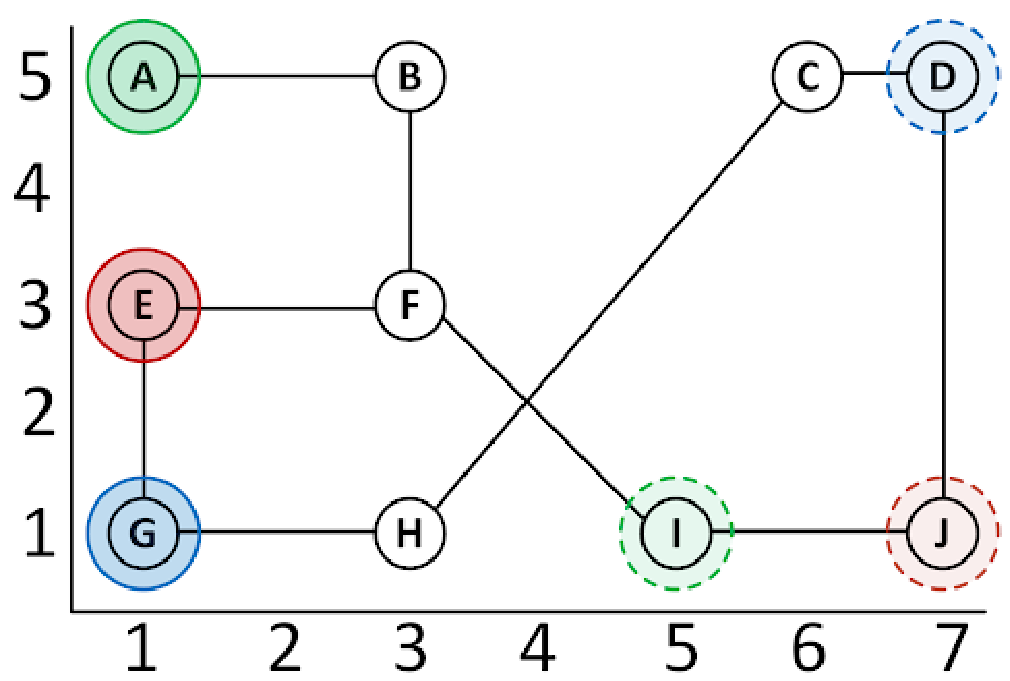
\includegraphics[width=0.6\columnwidth]{example_cropped.pdf}
    \caption{Our running example: a MAPF-E-CT problem with 3 agents.}
    \label{fig:example}
\end{figure}

Figure \ref{fig:example} shows an example of the problem. Small circles with the letters inside them denote graph vertices, e.g. vertex $A$ corresponds to a point with the coordinates $(1, 5)$, straight line segments between vertices depict edges, e.g. vertex $C$ is reachable from $H$ by following the segment that starts at $(3, 1)$ and ends at $(6,5)$. Agents are depicted as colored circles. Initially green agent occupies vertex $A$, red agent -- vertex $E$ and blue agent -- vertex $G$. Their respective goals are $I$ (green agent), $J$ (red agent), $D$ (blue agent).


In this work we focus on finding cost-optimal solutions. 
To define cost-optimality of a MAPF-E-CT solution, we first define the \emph{cost} of a plan $\pi_i$ to be the sum of the durations of its constituent actions. 
Several forms of solution cost-optimality have been discussed in \ac{MAPF} research. Most notable are \emph{makespan} and \emph{\ac{SOC}}, where the makespan is the max over the costs of the constituent plans and \ac{SOC} is their sum. The problem we address in this work is to find a solution to a given problem 
that is optimal w.r.t its \ac{SOC}, that is, no other solution has a lower \ac{SOC}. 

%As said before, typically, stating the MAPF problem begins with introducing the graph and constraints related to how agents are allowed to move on that graph. On the contrary, we wish to describe how agents and their moves are modeled in non-constrained environment (i.e. in 2D or 3D) and only then introduce a graph discretization of the problem.

%Consider a group of $n$ homogeneous agents operating in the shared environment which is a closed subset of the Euclidean 2-dimensional or 3-dimensional space, e.g. a bounded rectangle $W \in \mathbb{R}^2$. Without the loss of generality we will assume 2D workspace further in the paper. The environment is composed of the free space and the obstacles: $W = W_{free} + W_{obs}$. All agents have the same shape and size and each agent is characterized by its position $\textbf{p}=(x, y)$. An agent can move from one location to the other following an arbitrary shaped curve (line segment in the simplest case) connecting the move's endpoints.

%We assume that the two collision detection functions are given:
%\begin{itemize}
%    \item the one that detects collision w.r.t. static obstacles:
    
%    $col_{st}: W \rightarrow \{true, false\}$;
%    \item the one that detects inter-agent collisions:
    
%    $col_{ia}: W \times W \rightarrow {true, false}$.
%\end{itemize}

%In the simplest case, e.g. when the circular agents are considered, $col_{st}$ returns true if the distance between the position of an agent and the closest point in $W_{free}$ is less than the agent's radius; and $col_{ia}$ returns true if the distance between the positions of two agents is less than the sum of their radii.

%The path for an agent $i$ is defined as the mapping of the timeline to the workspace: $\pi: T \rightarrow W$, where $T=[0, + \infty)$.

%This definition of the path is the ``most unconstrained one'' as no limitations are imposed on how the agent might move, i.e. all sorts of acceleration/decelleartion are allowed, instantaneous direction changes are allowed, no constraints are imposed on the curvature of the path etc. Practice-wise this assumption never holds as only certain types of moves can be performed by the agents due to kinematic/dynamic constraints. Thus it is natural to introduce a notion of action and to constrain a path to be composed only of the actions in a certain order. Formally, action is, like a path, a mapping from time moments to workspace: $a: [t_b, t_e) \rightarrow W$, where $t_b, t_e \in T$ and $t_e<t_b$. And the path can now be defined as a sequence of actions: $\pi = \langle a_1, a_2, ..., a_k\rangle$, s.t. $t_e(a_j)=t_b(a_{j+1}$ and $a_j(t_e)=a_{j+1}(t_b)$. The conditions insure that the consecutive actions are well-aligned in time-space, i.e. the next action starts immediately after the previous one and in the same location of the workspace.


%We are considering cooperative pathfinding for non-point translating non-rotating agents in 2D workspaces. we consider all agents (1) to be of the same shape and size, i.e. open disks, (2) to move with the same (constant) speed, and (3) to be constrained to the same roadmap of the environment, i.e. there is a single graph $G=(V, E)$ whose vertices correspond to the locations agents can occupy (and wait in them) and edges correspond to straight-line trajectories the agents traverse when moving from one location to the other. Inertial effects are neglected and agents start/stop moving instantaneously. Duration of a move is translation speed times the length of the edge. Duration of the wait action can be any positive real number. 
%Prior work referred to this setting as \mapfr~\cite{walker2018extended}.
%Having that said, the problem we are considering is analogous to the one introduced by Walker et al.~\shortcite{walker2018extended} and dubbed \mapfr.

%Note that the \ccbs algorithm we propose in this work is not limited to assumptions (1), (2), and (3) described above, e.g., it can handle agents moving with different speeds, using different roadmaps, and having complex shapes and sizes. We make these assumptions only to simplify exposition. % provided with the appropriate collision detection procedure. It’s also extensible for 3D environments.Assumptions \textit{i}, \textit{ii}, and \textit{iii}For the sake of simplicity \konstantin{i think we need to say the following somewhere: may be here in text, may be in the footnote, maybe in the next section}Please note that the algorithm we are about to propose is not limited to \textit{i}), \textit{ii}) and \textit{iii}) assumptions, e.g. it can handle open-disk agents moving with different speeds and each of them using its own roadmap of the environment. Moreover it can be used for agents with different (complex) shapes and sizes provided with the appropriate collision detection procedure. It’s also extensible for 3D environments.

%The set of vertices $V$ represents a set of locations that the agents can occupy. We assume that any two agents, when standing still, can occupy any two vertices in the graph without colliding, i.e. their bodies will not overlap. For graphs based on grids and disk-shaped agents, this means the radius of every agent is less than or equal to half of the cell size.
%\begin{figure}
%\centering
%    \centering
%    \includegraphics[width=0.75\columnwidth]{RegularGraph.png}
%    \caption{}
%    \label{fig:reggrapph}
%\end{figure}
% Agents' actions
%When an agent is at a location $v\in V$, it can either  perform a \emph{move} action or a \emph{wait} action. 
%A move action moves the agent along an edge $(v,v')\in E$, and a wait action means the agents stays in $v$. 
%Every action has a \emph{duration}. The duration of a move action is the weight of the edge the agent is traversing. The duration of a wait action can be any positive real value. Thus, every agent has an infinite number of wait moves in every location. 
 
%\roni{I am missing more about the geometric prospective of the domain.  	That is, instead of a graph, the domain is actually represented by some terrain,  	and the graph is just set on that terrain. Probably there's such a definition in prior work on any-angle stuff.}





% END OF COPY AND PASTE FROM WORKSHOP PAPER


\subsection{Action execution in continuous time and space}
\textbf{K: This section might be of some value (but not sure)}

The distinctive feature of the considered problem statement is that the agents execute the actions of their plans in continuous time and space. By saying so we mean that for every agent $i$ and its plan $\pi_i$, and for every moment $t \in T=[0, +\infty)$ there exist a distinct $(x, y)$ location on the edge (or vertex) of the graph that is occupied by $i$ at $t$. In other words we are not blocking the edge entirely for the time the agent is traversing it.

Consider an example depicted on Figure \ref{fig:example} and assume the plan for the blue agent is $G \rightarrow H \rightarrow C \rightarrow D$ without any waits. Then, assuming that the moving speed equals 1, the agent will start traversing the edge $H \rightarrow C$ at time 2 and at time moment, say, $3.3$ it will be at the $(XXXX, YYY)$. This means that other agents, e.g. the red one, can be at this time moment anywhere on the edge $F \rightarrow I$ (the edge is not blocked), as the distance between the center of the blue agent and any point on the edge $F \rightarrow I$ is greater that $2r=2*0.5=1$.

\textbf{K: Maye some picture here showing (by the arrow) the position of the blue agent at time 3.3}
